% 2023本郷祭 マイコン部 部誌 「マイコンHONGOMagazine」 TeXテンプレート

% =環境設定=

\documentclass[b5paper,9pt,platex,dvipdfmx]{jsarticle}

% 数式
\usepackage{amsmath,amsfonts}
\usepackage{bm}

% 画像
\usepackage[dvipdfmx]{graphicx}
\usepackage{float}

% 段組
\usepackage{multicol}
\setlength{\columnseprule}{0.3pt}

% 余白
\usepackage[paper=b5j,truedimen,margin=15truemm,dvipdfmx]{geometry}

% ページ番号を削除
\pagestyle{empty}

% ソースコード環境
\usepackage{listings,jlisting}
\usepackage{ulem}
\lstset{
  basicstyle={\scriptsize\ttfamily},
  identifierstyle={\scriptsize},
  commentstyle={\smallitshape},
  keywordstyle={\scriptsize\bfseries},
  ndkeywordstyle={\scriptsize},
  stringstyle={\scriptsize\ttfamily},
  frame={tb},
  breaklines=true,
  columns=[l]{fullflexible},
  numbers=left,
  xrightmargin=0zw,
  xleftmargin=0zw,
  numberstyle={\scriptsize},
  stepnumber=1,
  numbersep=1zw,
  lineskip=0.5ex
}
\renewcommand{\lstlistingname}{リスト}

% 枠付き文字(引用文)
\usepackage{fancybox}
\usepackage{ascmac}

% URL
\usepackage{url}

% ルビ
\usepackage{okumacro}

\usepackage{ascmac}

% 書きたい内容に合わせてお好きなパッケージを導入していただいて構いませんが、外部パッケージは提出時に必ず合わせて提出してください。
% また、そのパッケージを使用している部分には必ずコメントをしてください。

% =環境設定ここまで=

\begin{document}

% =タイトル=
\title{今日からできる!簡単お手軽エミュレーション}
\author{wattz麻呂}
\date{\today}
\maketitle
% 初めのページのページ番号を削除(\maketitleの影響を回避)
\thispagestyle{empty}

% ここではページごとに段組しています。大きく画像を表示したいときなどは以下を \begin{multicols}{3} 、\end{multicols}のように変更すると文章が終わった直後から空白になります
\begin{multicols*}{3}
  
% 以下本文
%\it  \sout{テックス完全に理解した} \sc
$こんにちは、中学部長wattz麻呂です。\\
今回は簡単お手軽にエミュレーションをしてみたいと思います。\\$
\begin{itembox}{index}{1}
エミュレーションとは?\\
{2}ディスクイメージの準備\\
{3}エミュレータのインストール\\
{4}OSのインストール\\
{5}余談宣伝
\end{itembox}
\section{エ
ミュレーションとは?}
 エミュレーション、というものを聞いたことがありますか?\\
恐らく、intelMacを使ってる方やソフト開発関係の仕事をしている方の中には聞いたことある人もいるかもしれません。\\
この記事においてエミュレーションもしくは仮想化とは、ざっくり言うと「実在するPC(OS)の上で別の仮想的なPC(OS)を実行する」\\
と言う行為を示します。(実は、エミュレートと仮想化は似て非なる別物なのですが、この記事においてそれはあまり重要な情報ではないので同じ、ということにしておきます)\\
元々「エミュレーション」とは英語の「模倣する・真似をする」と言う意味に由来する「emulate」を語源としているため、極論何かを模倣していればエミュレートしている、と言う扱いになります。\\
では、そのエミュレートは具体的にどういう所に役に立つのか、という点に話を移します。\\
それは,「実機では実行できない/したくないという作業を実機の代わりにやる」というものになります。\\
例えば、Macにおいてはexe(一般的なWindowsのアプリケのファイル形式)を開くことは基本的にはできません。\\
そこで、Macで仮想化ソフトウェアを使用してWindows(OS)を実行することでexeファイルを開く、という使い方です。(こっちの方がライトな使い方)\\
もう一つの例は、同じmacOSでも、意図的にウイルスに感染させる、などの実機ではやりたくない作業を仮想環境化でやればOSが破壊されようともエミュレータのファイルを消すだけでなかったことにする、という使い方です。\\
しかし、エミュレートできるOSは最近のものに限りません。\\
例えばWindows95や漢字Talkなどの太古の昔のOSでも(頑張れば)エミュレートすることもできます。\\
私がエミュレートをする理由も「昔のOSを見るため」という側面が大きいので、今回の記事では主にその目的でエミュレートします(我々からするとWindowsXPまでは太古のOSなので、古いOSということにさせてください..)\\
\section{ディスクイメージの準備}
自作PCを作ったことがある方は分かると思いますが、もちろんエミュレーターでのOSインストールでも、インストールする元のディスク(CD,DVDもしくはUSBなど)が必須です。\\
なので、そのディスクの用意から始めます。サンプルとして、今回はWindows7とMacOSX10.1をやってみたいと思います。\\
まずはディスクをisoイメージ化します。WindowsならImgBurnなどで、Macなら「ディスクユーティリティ」から作成します。\\
iso(ディスクユーティリティを使用する場合はcdr)ファイルの作り方は使用するソフトによって異なるので割愛させていただきます。\\
さて、isoファイルが準備できたところで次のセクションに移ります。\\
\section{エミュレータのインストール}
では次に実際にエミュレータをインストールしてみましょう。\\
エミュレータのアプリは、PCと同じ役割を果たすため、エミュレートする対象のPCがエミュレートしようとしているOSに対応していないとエミュレートすることはできません。\\
よって、アーキテクチャやbios/UEFIの異なるOS同士は共存しえない、という話になります。\\
今回はx86(x64)上のWindows7とPowerPC上のMacOSX10.1なので、別のエミュレータソフトが必要になります。セクションを分けて解説します。
\subsubsection{Windows7}
今回はx86ベースで動作するOSの例として、Windows7を採用してみました。\\
x86系統のWIndowsであれば、基本的にはこのやり方で動作すると思います。(Win98以前のOSはインストールにMS-DOSが必要)\\
ではまず、Windowsの場合は「VMware Workstation Player」を、Macの場合は「VMware Fusion」を公式サイトの指示通りにダウンロードしてください。\\
%スペック的に無理な場合はVirtualBoxでも大丈夫ですが、低速だったり色々不便なのでVMware製品の方を推奨します。\\
ダウンロードが済んだらインストーラーを起動します。\\
Windowsならば以下の画像のように出ると思うので、nextを押して、その後は脳死で「はい」をクリックしまくるとインストールが終了します。\\
インストールが終了したら、デスクトップ上にできたショートカット「VMware Workstation Player」をクリックして起動します。\\
起動したら、ライセンスの認証画面が出ると思うので、「個人向けライセンス」を押すと無料で使えます。(商用利用するためにはライセンス購入が必要)\\
Macの場合ならdmgファイルがインストールされるので、ダブルクリックでマウントしてVMware Fusionのアイコンをクリックし、起動すると自動でインストールが完了します。(途中でパスワードの入力を求められるかもしれません)\\
%\begin{figure}[H]
 % \centering
  %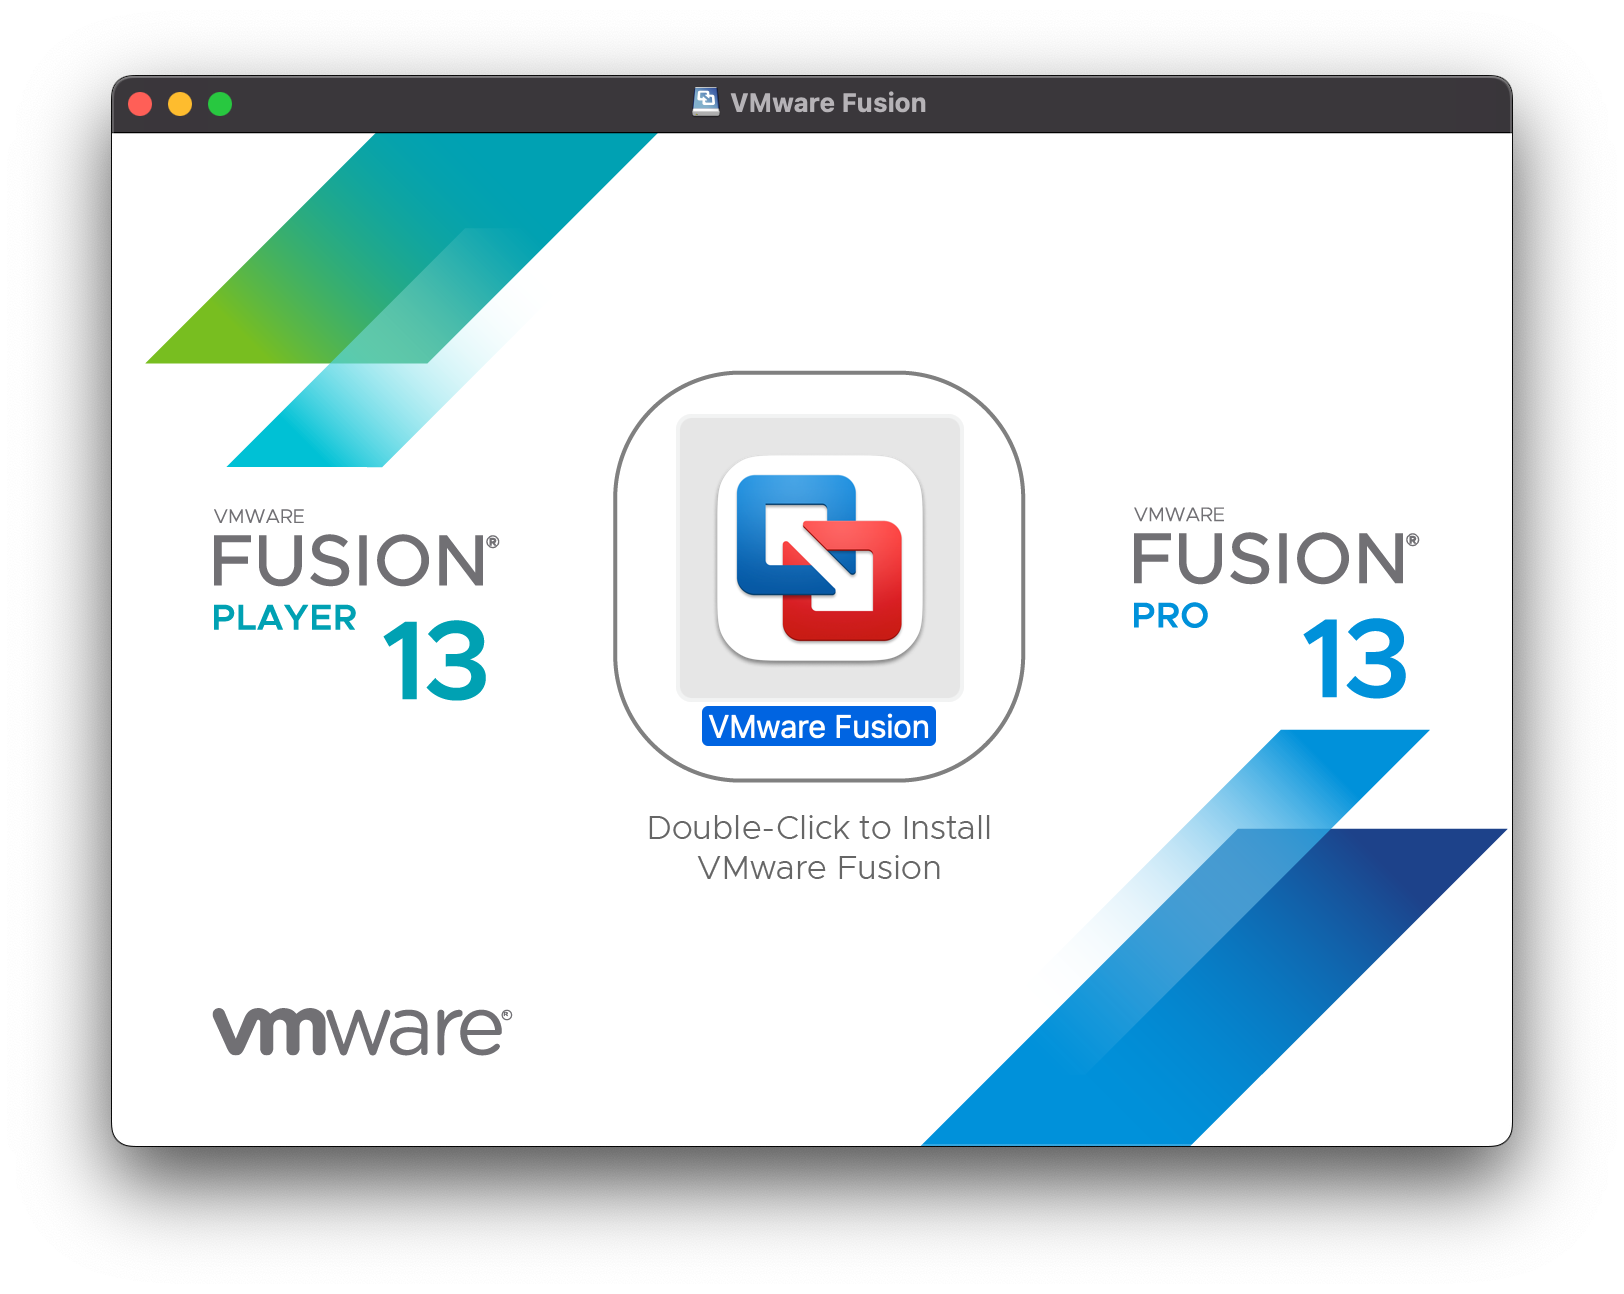
\includegraphics[width=5cm]{1.png}
  %\caption{画像は13ですが、個人的には12が非常におすすめです}
%\end{figure}
こちらの方はライセンスキーが必要なので、VMwareアカウントを作成して無料のライセンスキーを公式サイトより入手します。\\
以上でインストールは完了です。\\
次は、VMwareWOrksaionPlayerもしくはVMwareFusionで仮想マシンを作成します。\\
仮想マシンを作成(+)の項目よりOSのタイプを(今回は)Windows7に設定し、「次へ」を押しまくると最後に確認的なウインドウが出てくるので、「完了」を押します。\\
ディスクサイズはあとから調整できるます。ここで言うサイズとは、「仮想マシンで使用できる最大量」であり、実際のサイズは仮想マシンの中で使っている容量なので、120gbとかでも問題はありません。\\
メモリは多いほどいいですが、最大でも実際のメモリ容量の半分程度にしておきましょう。\\
\subsection{MacOSX10.1}
一応上級編としてQemuを使ってみます。\\
QemuはVMwareと同じようなエミュレータのようなものの一種で、主にコマンドラインベースなので難しめです。(多分)\\
VMwareFusion及びVirtualBoxでは同じアーキテクチャ(x86、arm等)のみしか仮想化できませんが、Qemuならばアーキテクチャが違ってもエミュレートできます。\\
今回やろうとしているMacOSX10.1はPowerPC上で動くOSであるため、x86環境上で実行するにはQemuを用いる必要があります。\\
余談ですが、Qemuはx86→PowerPCに限らず実行できます。例えばarm上のOSであるiPhoneOS1をx86上で実行することも可能という報告もありますし、m68kのA/UXなんかもエミュレート可能です。\\
QemuでMacOSをエミュレートする場合、エミュレート(模倣)する対象である機種が正確に決まっていたりします。\\
PowerPCの場合はPowerMacG3/G4、m68kの場合はQuadra800がエミュレートされ、OldWorldOS(MacOS9.2より前)をする場合ではPSエミュレータなどと同じようにROMイメージが必要です。\\
(macOSの場合は)コマンドラインのアプリであるため、本来は自らでビルドすべきなのですが、web上で拾ってくるのも手です。(私はemaculation.comでダウンロードしています)\\
自分でビルドする場合は公式サイトqemu.orgを参考してください。\\
今回の例ではemaculation.comでビルドされたファイルを使用して行います。\\
ダウンロードしたzipファイルを解凍して中のフォルダを見ると、以下のようになるはずです。\\
\begin{figure}[H]
  \centering
  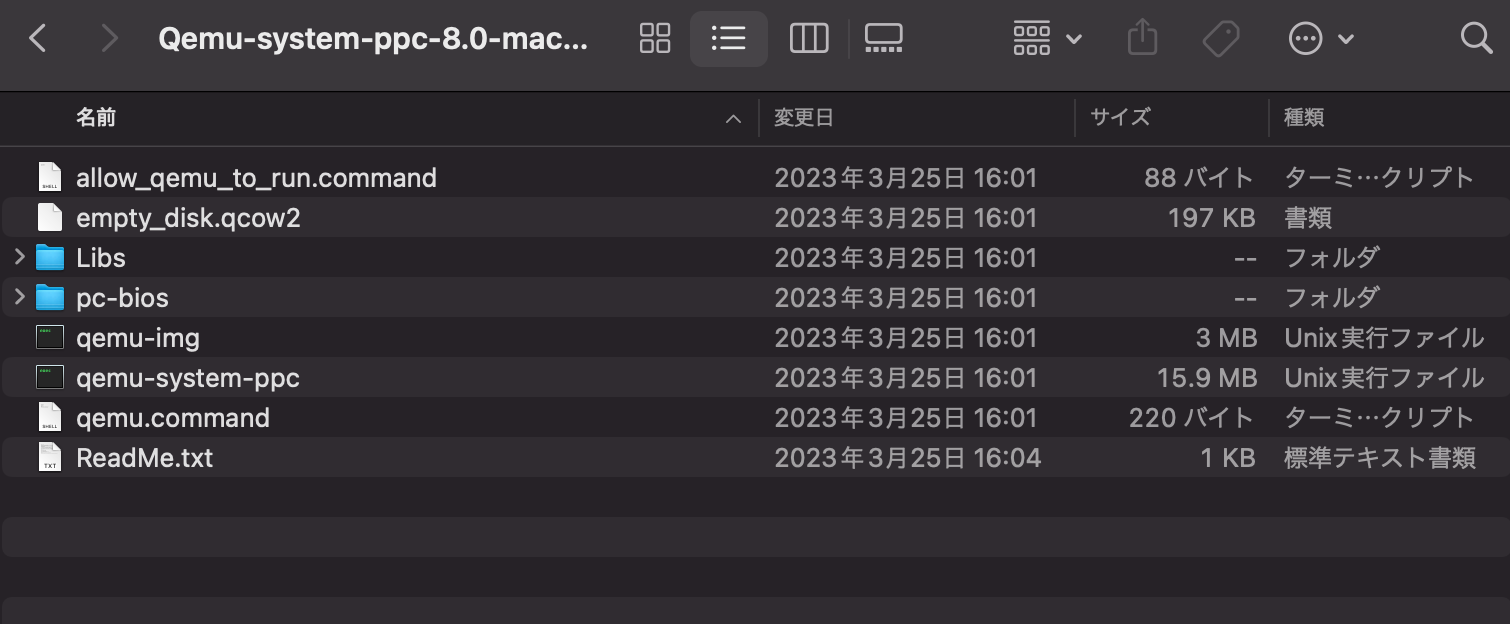
\includegraphics[width=4cm]{2.png}
  \caption{}
\end{figure}
まずは、中に入っているqemu.commnadもしくはqemu.batを編集します。\\
権限がない場合は、sudo chmod +x(もしくは777) qemu.commandへのパスとターミナルに入力します。\\
%次に、
%\begin{itembox}
%xattr \- c allow\_ qemu\_ to\_ run\. command
%\end{itembox}
%、エラーを吐かなければ
%\begin{itembox}
%sudo ./allow_qemu_to_run.command
%\end{itembox}
%と唱えます。\\
%sudoコマンドを実行するとパスワードを欲求されます。\\
mac版のqemu.commandを参考にして解説します。\\
\begin{itembox}{qemu.command}

cd "\$(dirname "\$0")"

./qemu-system-ppc \verb|\| \\
-L pc-bios \verb|\| \\
-M mac99 \verb|\| \\
-display cocoa \verb|\| \\
-m 512 \verb|\| \\
-boot d \verb|\| \\
-drive\ file=MacOS9.2.iso,format\\
=raw,media=cdrom \verb|\| \\
-drive\ file=MacOS9.2.img,format\\
=raw,media=disk \\
\end{itembox}
以上のファイルの意味を説明します。\\
Windowsの場合は\verb|\|を¥と読み替えてください。\\
\begin{itembox}{script}
  cd "\$(dirname "\$0")"\\
\end{itembox}
bashシェルスクリプトであることをmacOSへ宣言します。windowsの場合は代わりにqemu-system-ppc.exe と記述します。\\
\begin{itembox}{script}
-L pc-bios
\end{itembox}
使用するbiosのファイルの位置を定義します。\\
\begin{itembox}{script}
-M mac99,via=pmu 
\end{itembox}
Macのタイプなどを指定します。mac99はPowerMacG4、g3beigeはベージュ色のPowerMacG3をエミュレートします。(g3beigeは滅多に使いませんが、一部使うところもあります。例えば、Rhapsodyという\sout{闇に葬られた}OSをエミュレートするには-M g3beigeを使う必要があったり...)\\
via=pmuはマウスとキーボードの接続タイプで、via=pmu-adbやvia=cudaなどのオプションがあります。(滅多に使いませんが)\\
\textbf{今回は、マウスカーソルが動かないのでvia=pmuの部分は削除してください。}\\
\begin{itembox}{script}
-display cocoa 
\end{itembox}
一部サイトでは-display sdlと記述されていますが、最新版ではsdlはサポートされなくなったので、cocoaで実行してください。(MacOSの場合)\\
\begin{itembox}{script}
-m 512 
\end{itembox}
メモリの大きさをMB単位で指定します。2048mb(2GB)以下である必要があります。(PowerMacG4の最大搭載量)\\
\begin{itembox}{script}
-boot d
\end{itembox}
起動元を指定します。cに変更するとハードディスクから起動可能です。\\
\begin{itembox}{script}
-drive file=MacOS9.2.iso,format\\
=raw,media=cdrom \ \\
-drive file=MacOS9.2.img,format\\
=raw,media=disk 
\end{itembox}
エミュレートに使うファイルのパスを記述し、デバイスのタイプを指定します。\\
media欄はcdrom及びdiskが使えます。cdromはCDイメージ(iso,cdr)diskはハードディスクイメージ(img,qcow2,vmdk等)です。\\
\\
以上のように編集したら、先程用意したMacOSXのインストールディスクをMacOS9.2.isoとリネームして同じファイル内に入れます。\\
次は、qemu-imgを使用してディスクイメージの作成をします。\\
cmdもしくはターミナルを開き、qemu-system-ppcのディレクトリまで移動します。\\
そうしたら、
\begin{itembox}{script}
./qemu-img create raw -o size=2G MacOS9.2.img
\end{itembox}
と唱えます。./qemu-imgとはフォルダ直下にある実行ファイルの名称で、createとはqemu-imgの機能の一つです。\\
createは「ディスクを作成する」というコマンドで、create (フォーマット) -o size=(作成するサイズ) (ディスクファイルの名称).(拡張子)という形式です。\\
フォーマットではraw(信頼性が高く、macOSホストならそのままマウントできるが作成するサイズと実際のサイズが同じ容量になる。)、qcow2(qemuの仮想ディスクファイル、ゲストで使った分しか容量を食わない)、vmdk(VMwareFusionで使用される形式)、vdi(VirtualBoxで使用される形式)などが使用できます。\\
作成するサイズはなんでもいいですが、rawを使う場合は120gbで作成すれば120gb食うような感じなので、ゲストOSのバージョンによって変更しましょう。\\
MacOS9なら2GB、MacOSX10.0~10.3なら8GB、MacOSX10.4/10.5/10.6ベータなら12GBぐらいあれば安心です。(もしゲストOSで他のソフトを動かすなら、もっと多くする必要があるかもしれません。サイズは後から変更可能なので、多めに作っておいて損はありません。)\\
ファイル名は何でもいいですが、今回はデフォルトのqemu.commandに基づきMacOS9.2.imgとしました。拡張子はフォーマットと揃えた方がいいことのほうが多いので、そこだけ注意しておきましょう。\\
また、ディスクは一つでなくてはいけないとは限らないので、必要に応じて追加してください。(qemu.commandを変更しなければいけませんが)\\
これでひとまずは準備完了です。\\
\section{OSのインストール}
では実際にOSのインストールを行います。\\
\subsection{Windows7}
以下の画像のようなCDのマークがあり、それを押して仮想ディスクファイルを選択して、仮想マシンに接続します。\\
\begin{figure}[H]
  \centering
  
\includegraphics[width=4cm]{3.png}
  \caption{ここのバーの配置は変更可能です}
\end{figure}
そして、起動させます。画像のように起動しなかったらそのディスクはOSのインストールディスクではないか形式が合っていない可能性があります。\\
起動すれば、お馴染みのWindowsマークが出現し、OSのインストーラが起動します。\\
\begin{figure}[H]
  \centering
  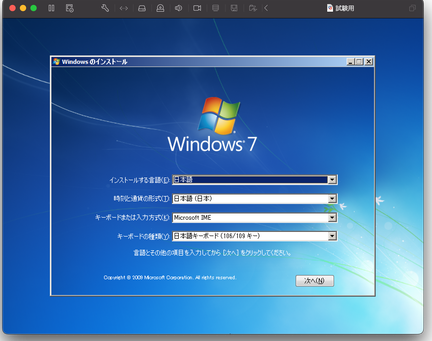
\includegraphics[width=4cm]{win7-cd.png}
  \caption{windows7の画面}
\end{figure}
「次へ」を押し、「今すぐインストール」を選択し、ライセンスに同意します。\\
次に、インストールするボリュームの決定に入りますが、実機と同じく非割当の項目を選択します。これは実機のハードディスクではなく、セットアップ時に作成した仮想ディスクなので躊躇なくフォーマットして大丈夫です。\\
インストールが始まったらしばらくやることがないので待機してましょう。(数回再起動します)\\
プロダクトキーの入力ですが、Windows7以降はスキップ可能\&後でどうせ有効化するために電話で認証をしなくてはいけないのでスキップで構いません。\\
で、諸々の初期設定を済ませ、デスクトップが写ったらVMwareToolsのインストールを行っていきます。\\
VmwareToolsとは、ゲストOSの設定をするもので、これを入れるとOSの解像度がいじれるようになったり、ホストOSとファイルのやりとりが簡単に出来るようになる便利ツールです。\\
メニューバーより、仮想マシン/ 「VMwareTools」よりインストールできます。(仮想マシンにCDドライブが接続されていて、空の場合)\\
一部のOS(Windows95/2000までのNT系統)やサポートされていないmacOS系などはVMwareToolsを当てるのに一筋縄ではいかない可能性もあります。\\
仮想ディスクを挿入したら自動的にインストールが始まります。\\
インストールが終了したら再起動して、ライセンスの認証をします。\\
仮想マシンのwifiを切り、コントロールパネル/システムより「今すぐライセンス認証をする」を押しましょう。\\
ここで、「ライセンス認証サーバーの接続に失敗しました」などと出るので、他の選択肢を表示し、「電話でライセンス認証をする」をクリックし、ウインドウの表示に従います。\\
WindowsVista等一部WIndowsでは「この地域では電話でのライセンス認証はサポートされていません」と出ますが、0120-801-734へダイヤルすれば認証できます。\\
以上で終了です。お疲れ様でした。\\
\subsection{MacOSX10.1}
ではMacOSXの方をインストールします。\\
前提としてMacOSは基本的にMacでしか起動できないようになっていて、基本的にOSはプリインストールされているため、ライセンスの認証が不要です。\\
なので、以上のライセンスが云々という面倒な作業は必要ありません。\\
では、実際にインストールをしましょう。\\
先程起動する準備は整ったので、qemu.commandをダブルクリックして起動します。\\
「開発元を検証できないため...」と出たらシステム環境設定の「セキュリティとプライバシー」パネルより「そのまま開く」を選択して起動します。\\
起動時に以下のように黄色の画面が出たら失敗です。「No valid  state has been set by load or init\-program.」と表示されたら使用可能なディスクではないということを示しています。\\
\begin{figure}[H]
  \centering
  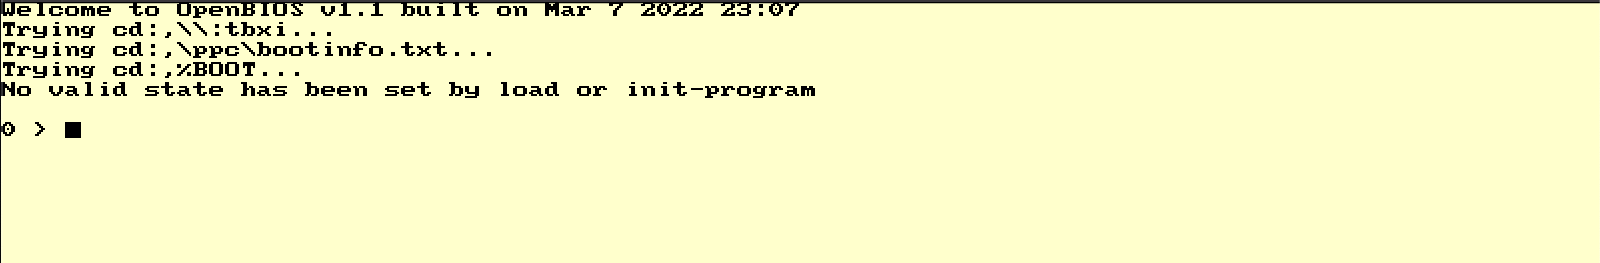
\includegraphics[width=4cm]{4.png}
  \caption{}
\end{figure}
起動に成功したら、以下の画像のように表示されます。(MacOSで伝統的なHappyMacです。10.2以降はグレーのリンゴマークが表示されます。)\\
\begin{figure}[H]
  \centering
  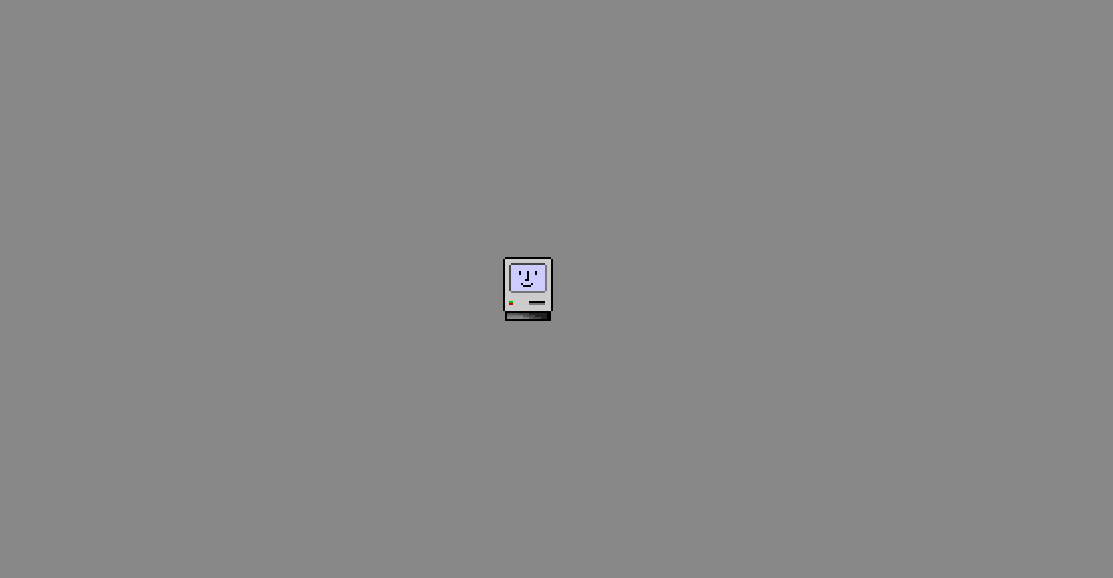
\includegraphics[width=4cm]{5.png}
  \caption{真ん中に出てくるのがHappyMac}
\end{figure}
起動したら、以下のようになるので、日本語を選択します。そしたら、メニューバーより「ユーティリティ」から「ディスクユーティリティ」を選択します。\\
\begin{figure}[H]
  \centering
  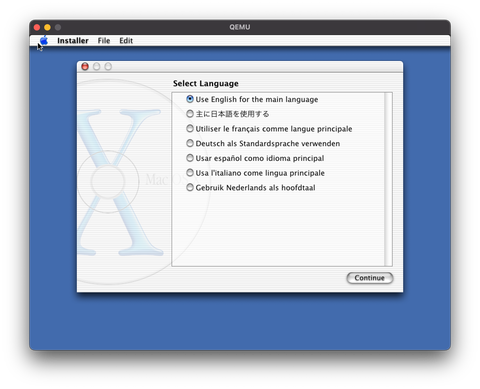
\includegraphics[width=4cm]{osx-cd.png}
  \caption{背景はOSにより異なる}
\end{figure}
そして、左側のバーよりハードディスクを選択して右下のボタンよりHFS+を選択してフォーマットします。(ディスクユーティリティのUIは\\
その後はライセンスに同意してインストールを開始します。\\
その後一回再起動しますが、再度cdから起動するのでシステム終了し、qemu.commandの -boot d の箇所を -boot c に変更します\\
そして再度qemu.commandをダブルクリックし、HDから起動し、セットアップをします。\\
一部の登録系はスキップできるので、「ようこそ」画面でcommand+Qを押すと登録系をスキップできます。\\
\begin{figure}[H]
  \centering
  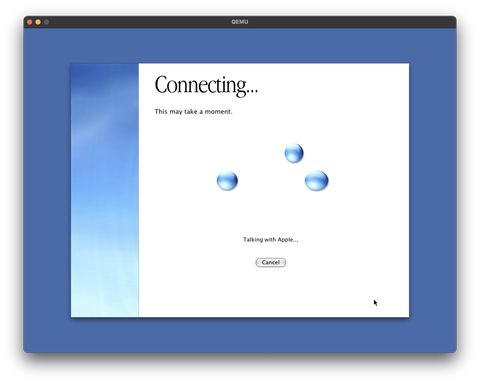
\includegraphics[width=4cm]{osx-connect.png}
  \caption{美しい。}
\end{figure}
左側に写ってる水面のエフェクトは、クリックすると波が立ちます。(自分でやってみてください)\\
設定を終えると以下のようにデスクトップ画面が表示されます。お疲れ様でした。\\
\begin{figure}[H]
  \centering
  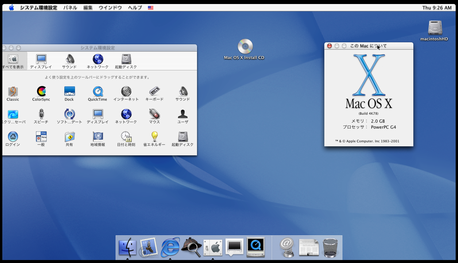
\includegraphics[width=4cm]{osxdesktop.png}
  \caption{やはりMacOSXは美しい。}
\end{figure}
\section{余談宣伝}
今回は簡単めな2種類を例にとって見ていきましたが、勿論一筋縄ではいかないOSもあります。\\
代表的な例がMacOSX10.4(intel)で、OS側が新しいCPUを認識しなかったり、機種固有のインストーラーしかないので、エミュレートがかなり難しかったりします。\\
そのような例はここに書き連ねるととても頁が足りないので、waltzmaro.blog.jp/ よりどうぞ。(宣伝)\\
個人的に一番むずいのはRhapsody5.6(現行macOSの前身)だと思います。興味のある方はやってみてください。\\
あと私事ですが、今回初めて\sout{テックス}\TeX を使用してみました。実に\sout{クソ}興味深かったので、これからもこれを使おうと思います\sout{大嘘}。\\
最後にRhapsody5.6とMacOSXDP3の画像乗っけて終わります。お疲れ様でした。\\
\begin{figure}[H]
  \centering
  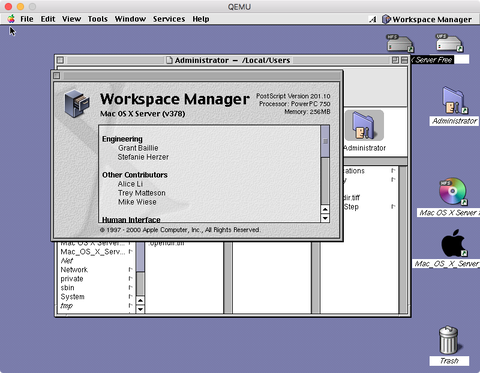
\includegraphics[width=6cm]{osx-rhapsody.png}
  \caption{Rhapsody5.6}
\end{figure}
\begin{figure}[H]
  \centering
  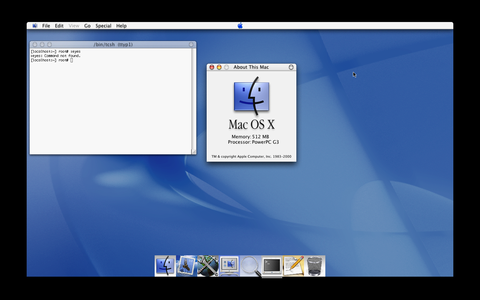
\includegraphics[width=6cm]{osx-dp3.png}
  \caption{DP3(Aquaが紹介されたバージョン)}
\end{figure}
以上です。\\
%世界に誇るSAITAMA

% ソースコードを挿入するときは以下のようにしてください
%\begin{lstlisting}[caption=Sample]
%mes "hello, world!"
%\end{lstlisting}



\end{multicols*}
\end{document}
